\chapter{Reti Neurali Convoluzionali per la Classificazione dei Melanomi}
\label{cap:nomePrimoCapitoloTesi}
\lhead{\textbf{\rightmark}}
In questo capitolo verranno presentate le reti neurali ed, in dettaglio, le reti neurali convoluzionali (note anche come CNN). Quindi sarà descritto il lavoro di addestramento della CNN e le scelte che sono state fatte in fase di progettazione.
\section{Reti Neurali Artificiali}
\label{sec:nomePrimaSezioneCapitolo}
\indent{
L'intelligenza artificiale ha contribuito in modo sostanziale a ridurre il divario tra gli esseri umani e le macchine. Una delle aree in cui l'intelligenza artificiale viene utilizzata è la Computer Vision. Una delle sfide più stimolanti è quella di consentire alle macchine di poter vedere, percepire e utilizzare conoscenza per effettuare numerose attività, tra cui la classificazione delle immagini. I progressi in campo di Computer Vision usando il Deep Learning hanno permesso di creare potenti algoritmi, tra cui le Reti Neurali. \cite{gori2003introduzione}
\newpage
Le \textbf{reti neurali artificiali (ANN)} sono modelli di calcolo matematico nati intorno agli anni ’40 del secolo scorso come riproduzione delle reti neurali biologiche. Esse svolgono funzioni di predizione ed elaborazione su insiemi estesi di dati basandosi sull’ipotesi dell’esistenza di pattern e interconnessioni fra le informazioni, costituite da neuroni artificiali, oggetto di studio.
\newline
Nella maggior parte dei casi, una rete neurale artificiale è un sistema adattivo che cambia la propria struttura in base a informazioni esterne o interne che scorrono attraverso la rete stessa durante la fase di apprendimento.
\newline
In termini pratici le reti neurali sono strutture non-lineari di dati statistici organizzate come strumenti di modellazione.
\newline
Esse possono essere utilizzate per simulare relazioni complesse tra ingressi e uscite che altre funzioni analitiche non riescono a rappresentare.
\newline
Una rete neurale artificiale riceve segnali esterni su uno strato di nodi (unità di elaborazione) d'ingresso, ciascuno dei quali è collegato con numerosi nodi interni, organizzati in più livelli. 
\newline
Ogni nodo elabora i segnali ricevuti e trasmette il risultato a nodi successivi.
\newpage
\section{Architettura delle Reti Neurali Convoluzionali}	
L'architettura delle reti neurali convoluzionali è inspirata dall'organizzazione della corteccia visiva animale,  i cui neuroni individuali sono disposti in maniera tale da rispondere alle regioni di sovrapposizione che tassellano il campo visivo. L'applicazione più popolare di una rete neurale convoluzionale è l'identificazione di cosa un'immagine rappresenta. 
\newline
Esse sono ampiamente utilizzate anche in applicazioni che processano media. 
\newline
	\begin{figure}[h]
	\begin{center}
		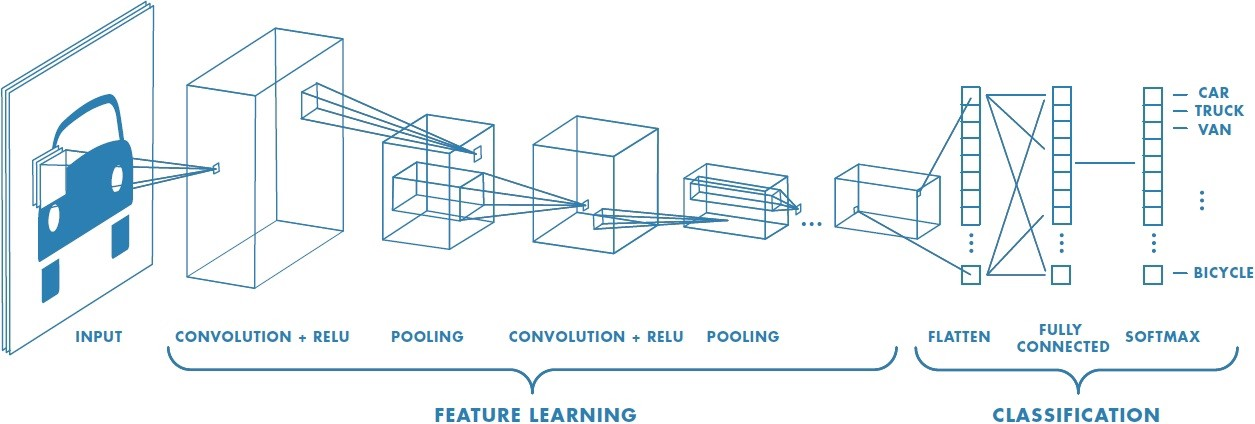
\includegraphics[scale=0.33]{figure/capitolo3/rnc.jpeg}
	\end{center}
	\caption{Esempio di costruzione CNN.}	
\end{figure}
\newline
Una Rete Neurale Convoluzionale è costituita da un blocco di input, uno o più blocchi nascosti, che effettuano calcoli tramite le funzioni di attivazione, e un blocco di output specializzato nella classificazione vera e propria. \cite{maiani2016applicazioni}
\newline
La principale differenza tra una rete neurale convoluzionale e una rete neurale classica è data dalla presenza dei livelli di convoluzione.
\newline 
L'input di una rete neurale convoluzionale è costituito da una sequenza di neuroni in grado di ricevere le informazioni dell'immagine che si vuole processare.
\newline
In questo livello, infatti, viene fornito il vettore dati che rappresenta i pixel dell'immagine in input. Nel caso di una immagine a colori RGB di dimensione 32 x 32 pixel, il vettore in ingresso avrà una dimensione 32 x 32 x 3, dove 3 rappresenta i tre colori.
\newline
Il livello convoluzionale è il principale della rete. 
\newline
L'obiettivo del livello convoluzionale è quello di individuare forme all'interno dell'immagine, come curve, linee, angoli, circonferenze o quadrati. Il livello convoluzionale fa uso di un filtro (o kernel), ossia una piccola matrice numerica che identifica una particolare struttura dell'immagine. Questa matrice si sposta sull'immagine di un determinato passo (o stride), iniziando dal punto dell'immagine in alto a sinistra.
\newline
Ogni volta che il kernel si ferma su un punto dell'immagine, dove per punto si intende la sottomatrice dell'immagine, viene calcolato il prodotto scalare tra il kernel e la sottomatrice. 
\newline
I risultati dei prodotti scalari formano l'immagine caratterizzata. Affinché l'immagine di uno strato abbia la stessa dimensione di quella dello strato precedente, è comune riempire l'immagine con zeri intorno al bordo, tale operazione viene detta \textit{zero padding}. 
\newline
Inoltre, ogni livello convoluzionale è seguito da una funzione di attivazione, la quale si pone come obiettivo quello di annullare i valori non utili dei livelli precedenti. 
\newline
La funzione di attivazione più usata è la ReLU (Rectified Linear Unit)\cite{agarap2018deep}. Questa funzione è non lineare ed è così definita: 
\begin{equation}
    f(x) = max(0,x)
\end{equation}
Un altro livello è il Pooling, che permette di ridurre l'immagine del livello convoluzionale precedente, al fine di ridurre il carico computazionale, la memoria, il numero di parametri e il rischio di Overfitting.
\newline
Il livello di Pooling usa semplicemente una funzione di aggregazione che calcola il massimo o la media dei valori dell'immagine che gli viene fornita in input.
\newline
Infine, è presente un livello FC (o Fully Connected) che effettua la classificazione vera e propria. \cite{Senn:2015}
\newpage
\section{Classificazione dei Melanomi con Deep Learning}
La metodologia utilizzata per la classificazione dei melanomi è basata su una tecnica di deep learning applicata alle immagini presenti nel dataset, in cui sono inseriti diversi tipi di malattie della pelle, inclusi i melanomi.
\newline
In particolare saranno utilizzate le reti neurali convoluzionali (CNN).
\newline
Per addestrare la CNN è stato utilizzato il dataset HAM10000.
La divisione scelta per il dataset HAM10000 consiste in:
\begin{itemize}
	\item 6705 nevi melanociti
	\item 1099 lesioni benigne
	\item 1113 melanomi
\end{itemize}
Per bilanciare i dati è stata effettuata una tecnica di data augmentation sulle immagini di melanomi.
\newline
Attraverso operazioni concatenate composte da flip orizzontali e verticali, rotazioni di 180, 90 e -90 gradi, ogni immagine originale del melanoma è stata utilizzata per generare sette immagini distinte, ottenendo così un totale di nuove 7.791 immagini che, sommate alle 1.113 iniziali, hanno formato 8.904 immagini di lesioni cutanee correlate al melanoma.
\newline
La CNN è stata addestrata con 100 epoche con un batch di 64 e utilizzando l'ottimizzatore Adam.
\newline
La rete neurale è stata costruita con 4 blocchi convoluzionali e un ultimo blocco per la classificazione. Il training set, il test set e il validation set sono stati formati considerando le percentuali 80\%, il 20\% del dataset iniziale e il 15\% del training set. 
I livelli convoluzionali utilizzano una dimensione del kernel pari a 5 e un passo di 1 e una regolarizzazione del kernel L2. 
Sono state utilizzate le Rectified Linear Units (ReLU) come funzione di attivazione per ogni livello convoluzionale e la funzione di attivazione Sigmoid nell'ultimo livello completamente connesso (FC) per avere una classificazione binaria del problema (0/1).
\begin{figure}[h]
	\begin{center}
		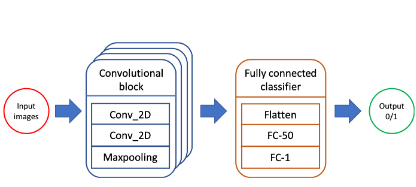
\includegraphics[scale=1]{figure/capitolo3/cnn1.png}
		\caption{CNN}	
	\end{center}
\end{figure}
\newpage
\subsection{Estrazione automatica della skin lesion}
L'estrazione automatica di una lesione cutanea in un'immagine è composta dai seguenti tre passaggi:
\begin{itemize}
	\item Hair Removal;
	\item Lesion Segmentation;
	\item Clinical Feature Segmentation;
\end{itemize}
\subsubsection{Hair Removal}
L'occlusione dei peli nelle immagini dermoscopiche influenza il funzionamento diagnostico della lesione cutanea.
Abbiamo utilizzato il rilevamento dei bordi \textbf{Canny} per la rimozione dei peli, che comprende due fasi:
\begin{itemize}
	\item nel primo, il pelo chiaro e il pelo scuro sono segmentati attraverso il rilevatore di bordi canny adattivo e la rifinitura da parte degli operatori morfologici.
	A seguito del rilevamento degli angoli di Canny, la soglia di Otsu è stata utilizzata come maschera per la rimozione dei peli al fine di ottenere un'immagine in bianco e nero. A questo punto è stato applicato un operatore di dilatazione per garantire una maggiore precisione nella cattura dei peli.
	\item Infine, è stato eseguito l'image inpainting, una tecnica che esegue una sorta di interpolazione per l'elaborazione di immagini digitali per ricostruire parti di immagini digitali danneggiate.
\end{itemize} 
\subsubsection{Lesion Segmentation}
La segmentazione mira a selezionare oggetti o regioni specifiche in una immagine sulla base di una proprietà scelta, ad esempio luminosità, colore e consistenza.
L'immagine viene convertita da RGB a scala di grigi e la parte viene separata dal suo sfondo (cioè, la pelle).
Il metodo Thresholding di TheOtsu viene utilizzato per eseguire automaticamente una soglia di immagine basata su clustering o la riduzione di un'immagine a livello di grigio in un'immagine binaria. L'algoritmo presuppone che l'immagine contenga due classi di pixel che seguono l'istogramma bimodale (cioè pixel in primo piano e pixel di sfondo); calcola quindi le soglie ottimali separando le due classi in modo che siano combinate lo spread (varianza intra-classe) è minimo. Si ipotizza che i bordi con un gradiente di intensità maggiore del valore massimo siano bordi reali, mentre quelli al di sotto del valore minimo non sono certamente bordi e quindi da scartare. 
\begin{figure}[h]
	\begin{center}
		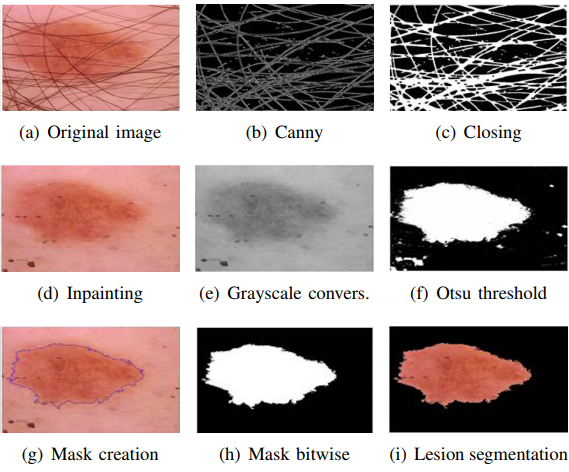
\includegraphics[scale=0.68]{figure/capitolo3/imagepro.png}
	\end{center}
	\caption{Preprocessing per ogni nevo.}	
\end{figure}
\newpage
\subsubsection{Clinical feature segmentation}
In questo caso è presente una segmentazione locale della lesione, evidenziando così le caratteristiche cliniche di una lesione come la consistenza, la forma e il colore.
\newline
Successivamente, è stato necessario ridurre l'eccessiva segmentazione, un tipico "problema" che si verifica nell'output della fase precedente. sfruttando una tecnica basata sulla media temporale e spaziale. In questo caso è stato utilizzato un filtraggio mediano che preserva i bordi rimuovendo l'eccessiva segmentazione e anche l'effetto di sfocatura.
\newline
Il filtro mediano consiste nel centrare una maschera, ordinare i pixel in modo crescente e assegnare il valore mediano al pixel del kernel.
\newline
Quindi, l'operatore AND binario bit per bit è stato applicato tra l'immagine generata e quella originale.
\newpage
\section{Addestramento}
È stata utilizzata la CNN 2D per eseguire una convoluzione spaziale bidimensionale sulle immagini. 
\newline
La CNN 2D è stata addestrata attraverso 100 epoche con una dimensione di lotto di 50 e utilizzando l'ottimizzatore Adam. 
La rete neurale è stata costruita con 4 blocchi convoluzionali (composti da strati 2D convoluzionali e Maxpool) e un ultimo blocco fully connected (FC) per la classificazione. 
\newline
Il training set, test set e validation set sono stati impostati considerando rispettivamente le percentuali 80\%, 20\% del set di dati iniziale e 20\% del training set.
\newline
I livelli convoluzionali utilizzano una dimensione del kernel di 3 e un passo di 1 e una regolarizzazione del kernel L2 per gli strati convoluzionali e densi. Sono state utilizzate le unità lineari rettificate (ReLUs) come funzione di attivazione per ogni livello convoluzionale e la funzione di attivazione sigmoide nell'ultimo livello FC per avere una classificazione binaria del problema. 
\newline
Abbiamo anche aggiunto due livelli di Dropout; uno dopo i layer Convolutional 2D e Maxpool pari a 0.25, e l'altro dopo il primo livello FC anch'esso uguale a 0.25.
}
